\pagestyle{fancy}
\chapter{Experimental protocol}
\label{Chap3}

In this part, we will describe the experimental protocol that was used for the realization of the structures and the setup for the measurements made.

    \section{Parameters}
    
        The following table describes the different tools used for the realization of the samples and shows the main parameters that have to be taken into account during the fabrication. The parameters in bold are the most influent.
        
       \vspace{0.5cm}
        \begin{graphe} 
        \centering
        \begin{tabular}{|c|c|c|}
        \hline
        \textsc{Step}&\textsc{Device}&\textsc{Parameters}\\
        \hline
        Resist deposition&Spinner&Rotation Speed, Acceleration, Time\\
        \hline
        Resist baking&Hot plate&Temperature, Time\\
        \hline
        Pattern design&EBL&\textbf{Dose}, \textbf{Shape(area)}, Resolution\\
        \hline
        Development&MIBK, MG, IPA&\textbf{Duration, Concentration}\\ 
        \hline
        Deposition of metal&Evaporator&\textbf{Angle}\\
        \hline
        Oxidation&Evaporator&\textbf{Pressure}, \textbf{Duration}\\
        \hline
        Plasma Etching&Plasma gun&\textbf{Duration}, Position, Power\\
        \hline
        Lift-off&Aceton&$\varnothing$ \\
        \hline
        
        \end{tabular}
        \caption{Steps of the process, tool or method used to realize this step and parameters involved by the step}
        \end{graphe}
        \vspace{0.5cm}
        
            
            The chip realized consists in twenty samples, with four different surface areas. It is thus possible to make a small statistic for the room temperature measurements.
                        
        \section{Experimental procedure}
        
            Here is the experimental procedure of the process. Based on 4 layers of MMA and one layer of PMMA and EBL dose from 2000 to 3000 $\mu$c/cm$^2$, according to the pattern in Fig. \ref{patternjunction}, the chip was dived 20s in MIBK, 20s in MG and IPA, to develop the exposure. In the evaporator, 20nm of Al are evaporated. To reproduce the native oxidation when exposed to air, the Al can be strongly oxidized with a pressure of 200mbar of O$_2$ during 10 min. After the strong oxidation, plasma etching is performed \textit{in situ} to get rid of the thick oxide layer. The tunnel barrier are made by exposition to O$_2$ at a pressure of 2mbar during 2min. Finally, 25nm of Cu are evaporated before diving the sample in acetone for the lift-off.
            In order to test the plasma etching, several realizations have been done, first to get some references (without plasma etching) :
            
            \indent - Clean contact  \\
            \indent - Strong Oxidation\\
            \indent - With tunnel barrier
                     
            Then we made samples with strong oxidation, then plasma etching, and finally either clean contact or with a tunnel barrier. An exhaustive table of the parameters used for each test can be find in Appendix \ref{parametertable}. Both room temperature and low temperature measurements are done, their goal are different. Room temperature measurements allows to check if the plasma really etches : the resistance of the samples should be similar to the resistance of reference samples. The low temperature measurements give us the quality of the junctions, especially the difference of quality between plasma etched samples and reference samples, which is not possible at room temperature.
            
            \begin{figure}
                \centering
                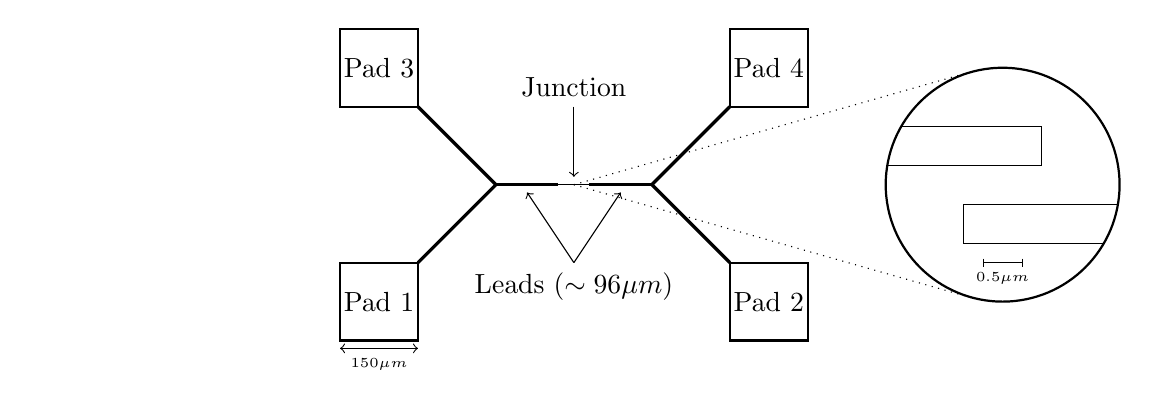
\begin{tikzpicture}[scale=0.99]
                    \draw [thick](0,0)--++(1,0)--++(0,1)--++(-1,0)--cycle;
                    \draw [<->] (0,-0.1)--(1,-0.1);
                    \draw (0.5,-0.1) node[below]{{\tiny $150\mu m$}};
                    \draw [thick](0,3)--++(1,0)--++(0,1)--++(-1,0)--cycle;
                    \draw [thick](5,0)--++(1,0)--++(0,1)--++(-1,0)--cycle;
                    \draw [thick](5,3)--++(1,0)--++(0,1)--++(-1,0)--cycle;
                    \draw [very thick](1,1)--(2,2);
                    \draw [very thick](1,3)--(2,2);
                    \draw [very thick](5,1)--(4,2);
                    \draw [very thick](5,3)--(4,2);
                    \draw [very thick](2,2)--(2.8,2);
                    \draw [very thick](4,2)--(3.2,2);
                    \draw (2.8,2)--(3.2,2);
                    \draw [->] (3,3)--(3,2.1);
                    \draw (3,3)node[above]{Junction};
                    \draw (0.5,0.5)node{Pad 1};
                    \draw (0.5,3.5) node{Pad 3};
                    \draw (5.5,0.5)node{Pad 2};
                    \draw (5.5,3.5)node{Pad 4};
                    \draw [->] (3,1)--(2.4,1.9);
                    \draw [->] (3,1)--(3.6,1.9);
                    \draw (3,1)node[below]{Leads ($\sim 96\mu m$)};
                    \draw [dotted,thin] (3,2)--(8.1,3.45);
                    \draw [dotted,thin] (3,2)--(8.1,0.55);
                    \draw [thick](8.5,2) circle(1.5);
                    \draw (7.2,2.75)--(9,2.75)--(9,2.25)--(7.02,2.25);
                    \draw (9.8,1.25)--(8,1.25)--(8,1.75)--(9.98,1.75);
                    \draw (8.25,1.05)--(8.25,0.95);
                    \draw (8.75,1.05)--(8.75,0.95);
                    \draw (8.25,1)--(8.75,1)node[midway, below]{\tiny{0.5$\mu m$}};
                    \draw [color=white](-4,2)--(-4,2.01);
                \end{tikzpicture}
                \caption{Pattern of the junctions}
                \label{patternjunction}
            \end{figure}
            
            \section{Oxygen cleaning}
            
            After heavy use of the plasma for etching, some troubles appeared and a cleaning of the gun with plasma oxygen was needed. After the cleaning, the etching power of the plasma seemed to have increased, and whereas ten minutes of plasma was needed in the first runs, the same etching time over-etches the sample after the oxygen cleaning (See Chapter \ref{Chap4}) and it has thus to be reduced.
             
            \section{Measurement setup}
            \subsection{Room temperature setup}
                            
Four-probe resistance measurements were realized thank to a probestation. The four-probe measurements make sense as it is the only way to measure the real resistance of the device, without parasite resistances (pads, wires). A schematics representing four-probes measurements is shown in Fig. \ref{Schéma4fils}. The probestation applies a voltage with an electrode and makes a slope from -100 mV to 100 mV, but measures the voltage $V_{sample}$ and the current $i_{sample}$ with two other electrodes so, the voltage and current measured are really these that cross the sample. The linearization of the I-V curve obtained directly gives the resistance of the sample, which is made through a matlab program.

\begin{figure}
            \centering
            \begin{circuitikz}[scale=0.9]
            \draw 
        (0,0) node[ground]{} 
            to [V,v=$DC$] (0,3)
            to [american resistor=$R_{wires}$, -*] (2,3)
            to [american resistor=$R_{pads}$, -*] (4,3)
            to [R=$R_{sample}$,i=$i_{sample}$] (9,3)
            to [american resistor=$R_{pads}$,-*] (11,3)
            to [american resistor=$R_{wires}$,-*] (13,3)
            to [ammeter, i=$i_{sample}$] (13,0) node[ground] {}
        
        (4,3) to [american resistor=$R_{Voltmeter}$, *-] (4,1)
            to [voltmeter, v_>=$V_{sample}$] (9,1)
            to [american resistor, -*] (9,3)
            ;
            \end{circuitikz}
            \caption{Four-probe measurements schematics}
            \label{Schéma4fils}
            \end{figure}
                
            \subsection{Low temperature setup}
                
                Measuring samples at low temperature is necessary to completely characterize the samples. First, it allows us to reach the superconducting state of Al (T$_C$=1.2K). Then, it reduces the thermal energy $k_BT$ so it reduces thermic transport which widen the electronic transitions.
               The samples are measured with two probes and not four like at room temperature. There are two main reasons, first the important parameter we want to get is $\dfrac{R}{R_{leak}}$ to check the quality of the junction, and this parameter will not be very affected by parasite resistance, since is is measured in order of magnitude : $R_{leak}$ is order of magnitudes higher than parasite resistances. Secondly, it is important to have some statistics, and the number of samples bounded for each cool down is limited, we thus make the choice to have statistics rather than few very accurate results. The measurements made are I-V curves with adjustements for the range of $V_{bias}$ : a large range for the tunnel current and a small range for the leakage current.
                
                                          
%         \begin{figure}
%             \centering
%             \begin{circuitikz}
%                 \draw 
%             (0,0) node[ground]{} 
%                 to [V,v=$DC$,v_>=$V_{meas}$] (0,3)
%                 to [R=5<\kilo\ohm>] (3,3)
%                 to [R=20<\ohm>,*-,v_<=$V_{bias}$] (3,0)
%                 node[ground] {}
%             (3,3) to [R=$R_{sample}$,i=$i_{sample}$] (8,3)
%                 to [ammeter, v^<=$V->I_{amplifed}$] (8,0) node[ground] {}
%             ;
%             \end{circuitikz}
%             \caption{Schematics of the set up for low temperature measurements}
%          \label{circuit}
%         \end{figure}
%         
                
                
                
                
                
                
            
